\chapter{Ontwerpproces}
\setheader{Ontwerpproces}

\section{Meetopstelling}
Om de directiviteit van de smartphone zo goed mogelijk te meten, wordt de impulsieresponsie van de microfoon gemeten in een anechoische kamer (ookwel dode kamer genoemd).
De metingen zijn verricht in de anechoische kamer op de faculteit TNW van de Technische Universiteit Delft.
In het midden van deze kamer wordt een boog met een straal van een meter opgesteld. Op deze boog is een luidspreker bevestigd, die over de boog kan worden bewogen.
De boog heeft een bereik van $-75^\circ$ tot $75^\circ$, waarbij de referentie $0^\circ$ de horizon is.

De telefoon wordt opgesteld op een turntable\footnote{Onderdeel van het op afstand bestuurbare B\&K 9640 turntable systeem.}, precies in het middelpunt van de boog.
Deze turntable kan op de graad nauwkeurig worden afgesteld.
Om op de boog de juiste graden in te stellen is het idee nu om een gradenboog op een A3-tje af te drukken en met een touwtje de hoek die de telefoon maakt met de speaker bepalen.
We gaan nog op 3ME / aan Henry den Bok (van de dode kamer) vragen of er een gemakkelijkere oplossing is.

%Keuze tafel / geen tafel / materiaal e.d.

Omdat we drie dagen hebben voor de metingen, zijn we beperkt in het aantal metingen dat we kunnen doen. Onze planning ziet er zo uit\footnote{Mocht de synchronisatie mislukken, dan gaan we de USB-microfoons gebruiken als back-up.}:
\begin{table}[h]
\begin{tabular}{|l|l|}
\hline
Maandagochtend & Opbouwen\\
Maandagmiddag & Meting met Nexus zonder tafel\\
\hline
Dinsdagochtend & Meting met Nexus met tafel (een keer face-up, een keer face-down)\\
Dinsdagmiddag & 14:30u - College Ethiek \& Techniek\\
\hline
Woensdagochtend & Meting USB-microfoon \\
Woensdagmiddag & Uitloop / meting aan HTC (keuze wel of geen tafel afhankelijk van andere resultaten)\\
\hline
\end{tabular}
\end{table}

Een andere overweging zijn de hoeken groter dan $75^\circ$ en kleiner dan $-75^\circ$, want daar is geen boog voor beschikbaar.
De telefoon onder een hoek op de turn-table zetten is geen optie, omdat dan de hoek veranderd met iedere verandering in de $\theta$-richting.
We zouden de turntable ook schuin (met bierviltjes o.i.d.) kunnen zetten (en de telefoon met dubbelzijdig plakband vastplakken) om de hoeken groter dan $75^\circ$ te bereiken. Hoeken kleiner dan $-75^\circ$ voor de telefoon in 'mid-air' kunnen we doen door te telefoon om te keren en dan de $+75^\circ$-opstelling te gebruiken.
Voor de telefoon op tafel is kleiner dan $-75^\circ$ niet mogelijk omdat de turntable dan op de plaats staat waar de speaker zou moeten zijn, maar het lijkt op het eerste oog ook niet nodig om lager dan $-75^\circ$ te meten als de telefoon op een tafel ligt.

\begin{figure}[h]
    \centering
    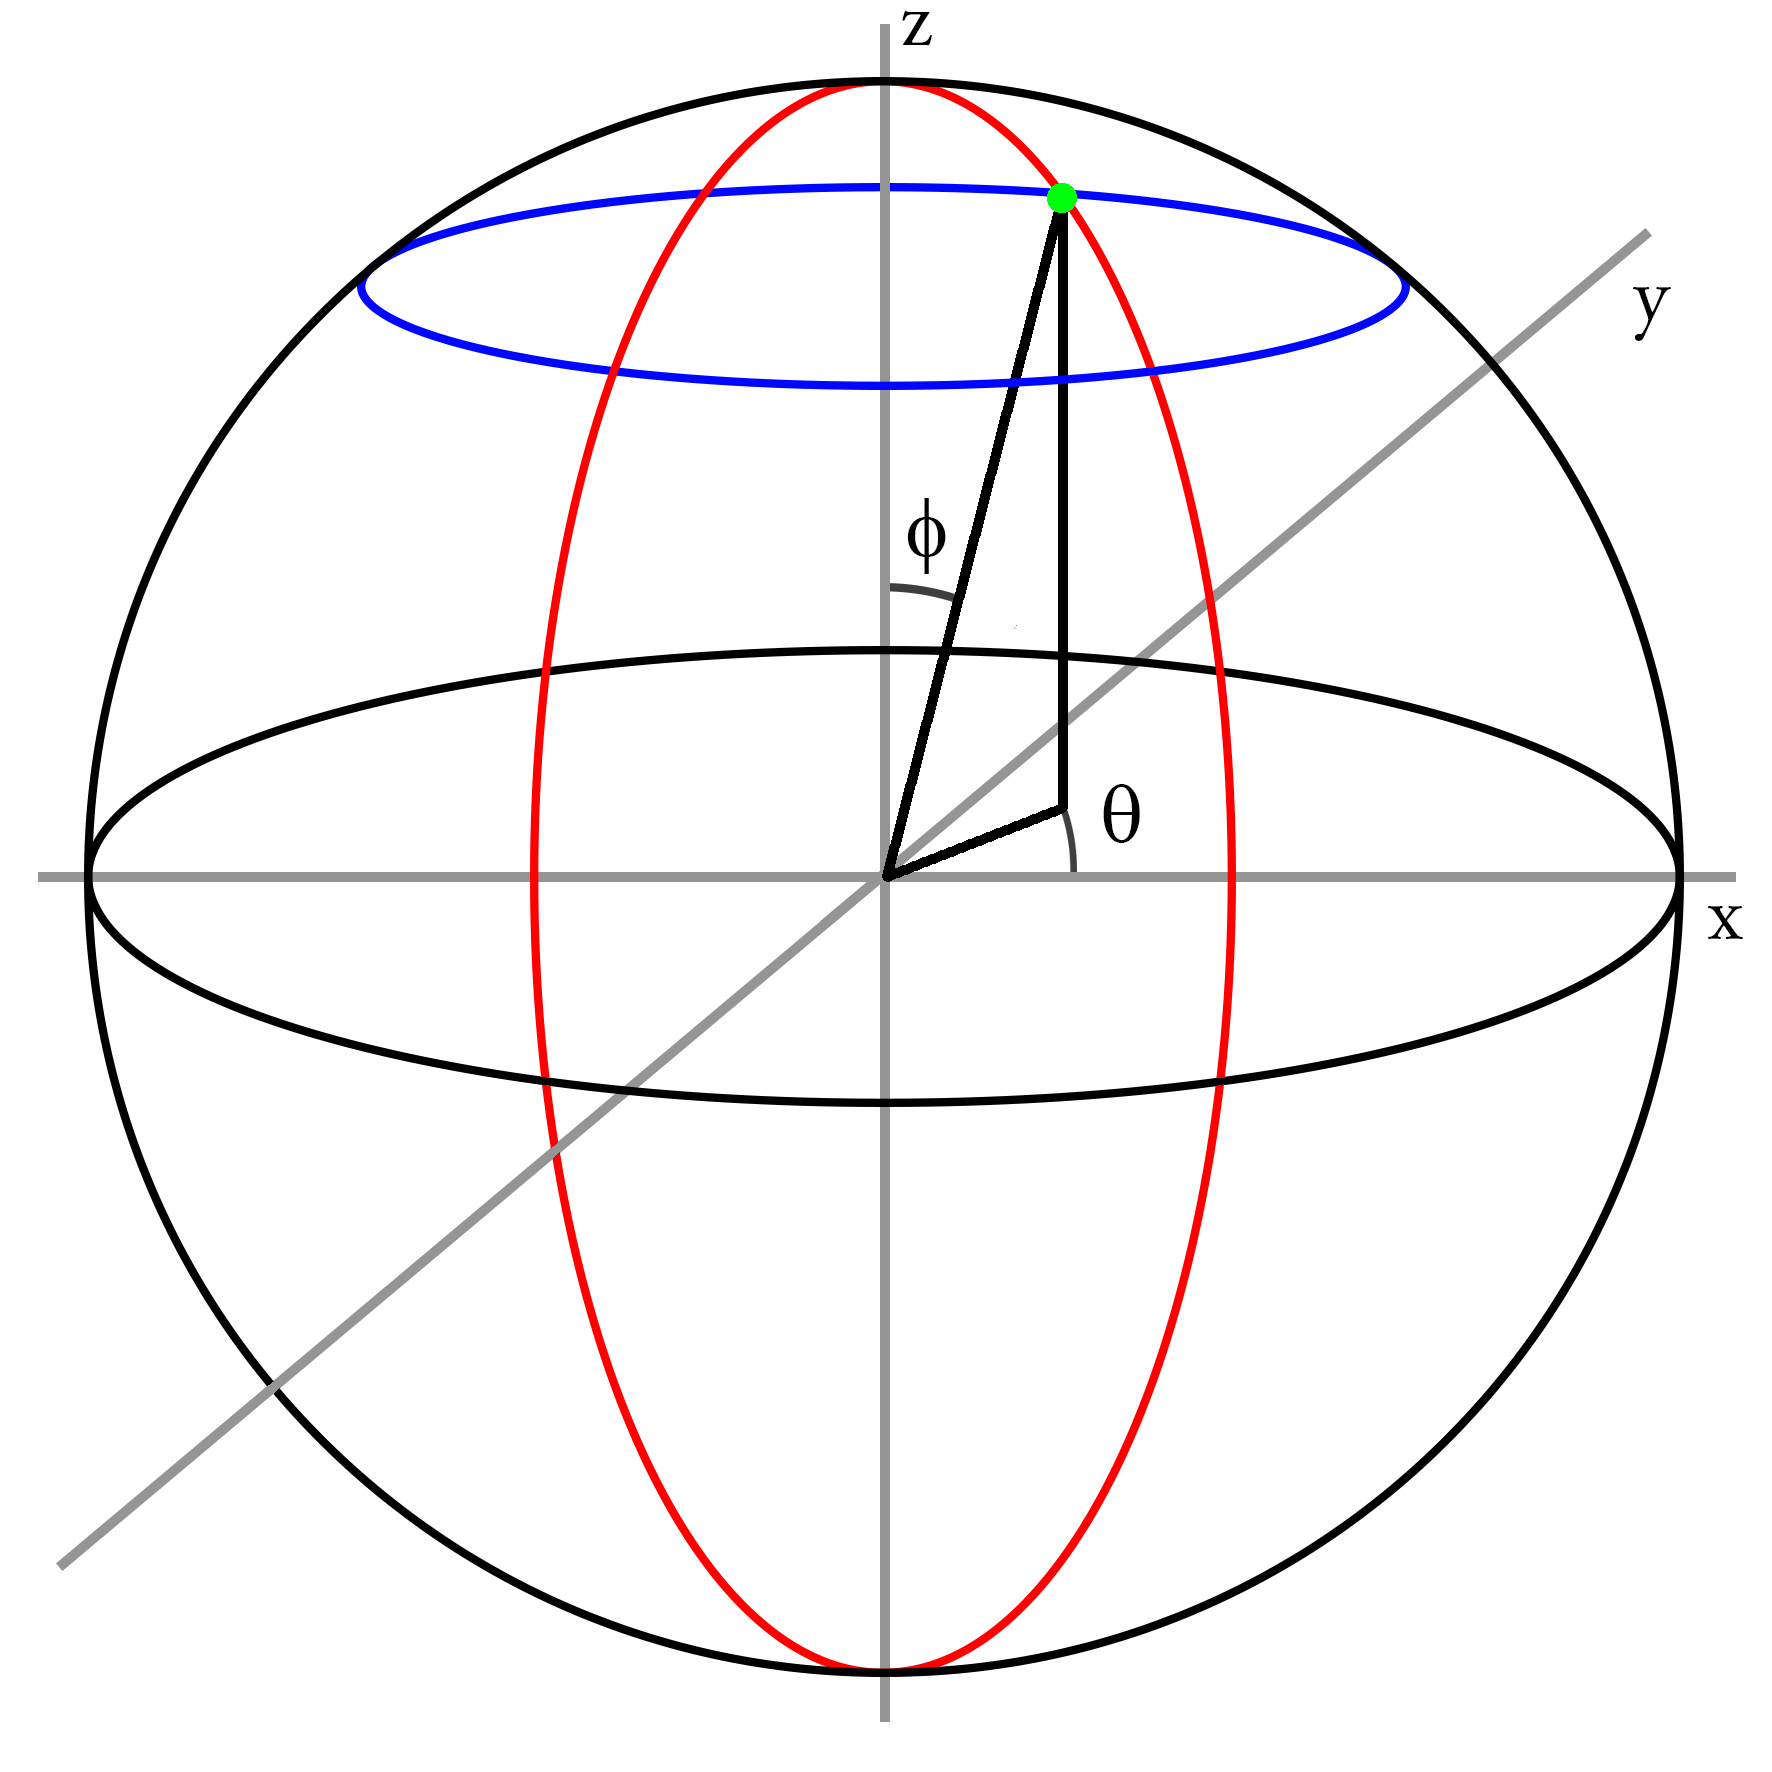
\includegraphics[width=8cm]{afbeeldingen/bol_definitie.png}
    \caption{De definities van verschillende namen op een bol:\\
    $\theta$ is de hoek tussen het punt en de $x$-as;\\
    $\phi$ is de hoek tussen het punt en de $z$-as;\\
    De rode lijn is een meridiaan;\\
    De blauwe lijn is een breedtegraad.}
    \label{fig:bol_def}
\end{figure}

\begin{figure}[h]
    \centering
    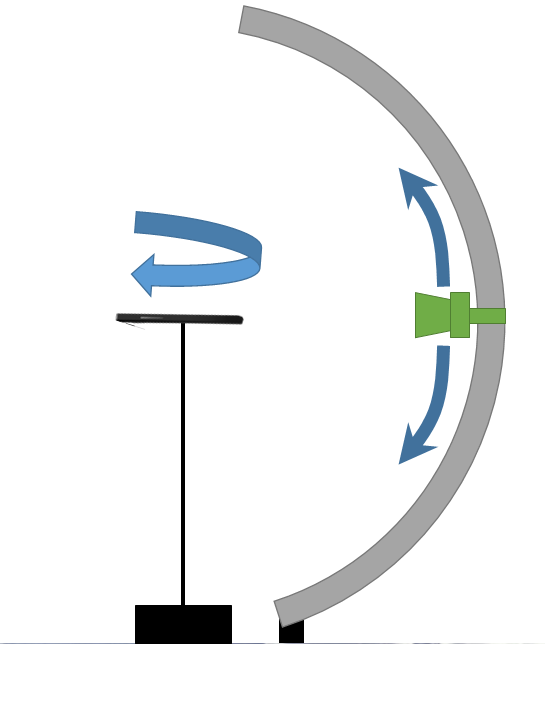
\includegraphics[width=8cm]{afbeeldingen/opstelling_pptx.png}
    \caption{Een schets van de meetopstelling}
    \label{fig:opstelling_pptx}
\end{figure}

%-----------------------------------------------------------------------------
\section{Bemonsteringsschema}
Er zijn veel verschillende manieren om een bol te bemonsteren \cite{Zhang2012575}.
De turntable kan worden aangestuurd door \matlab.
De afstelling over de boog moet echter wel handmatig gebeuren en daarom wordt er gekeken naar bemonsteringsschema's die zo min mogelijk handmatige handelingen vragen.

Om foutmarges te verkleinen, wordt er uitgegaan van een maximale afstand tussen twee meetpunten van een helft van de minimale golflengte (vergelijking \ref{eqn:ontwerp_afstandmin}).
Daarbij gaan we uit van een geluidssnelheid van $v_\text{lucht}=344$ m/s en een maximale frequentie in het menselijk stemgeluid van $f_{\text{stem}_\text{max}}=8$ kHz.
\begin{equation}
\label{eqn:ontwerp_afstandmin}
\Delta\ell_\text{max}=\dfrac{\lambda_\text{min}}{2}=\dfrac{1}{2}\dfrac{v_\text{lucht}}{f_{\text{stem}_\text{max}}}=\dfrac{344}{16000}=2.15\text{ cm}
\end{equation}
De bol waarop bemonsterd gaat worden, is de bol met als middelpunt de microfoon van de telefoon en als straal de lengte van de telefoon.
Binnen deze bol wordt het gedrag van het geluid be\"invloed door de telefoon en buiten deze bol maakt het niet uit welke bol je kiest, dus kiezen we de kleinste.
De(grootste) telefoon heeft een lengte van $\ell_\text{telefoon}=13.87$ cm, dus de lengte van de evenaar is dan $\ell_\text{evenaar}=2\pi\ell_\text{telefoon}\approx87.1$ cm.

%DUS ALS WE VERSCHILLENDE TELEFOONS GEBRUIKEN, NEMEN WE ALS LENGTE DE LANGSTE TELEFOON

Er zijn twee bemonsteringsschema's in overweging genomen vanwege het lage aantal verplaatsingen over de $\phi$ richting.
\subsection{Equiangular}
Dit bemonsteringsschema gaat uit van gelijke hoeken tussen de monsters.
Dit deelt de bol dus op een aantal lengte- en breedtegraden. In de $\theta$-richting zal er over $360^\circ$ een meting worden gedaan en in de $\phi$-richting over $180^\circ$. Daarom is het belangrijk dat het hoekverschil een gemene deler is van zowel 180 als 360. Er wordt dus ook over de evenaar gemeten, dit is de cirkel met de grootste afstand tussen twee meetpunten. Daarop moet dus gelden dat $\Delta\ell_\text{max}\geq\ell_\text{evenaar}\cdot\dfrac{360^\circ}{\Delta\theta}$. Daaruit volgt dat $\Delta\theta_\text{midden}\leq\dfrac{360^\circ\cdot\Delta\ell_\text{max}}{\ell_\text{evenaar}}\approx8.9^\circ$. De grootste gemene deler van 360 en 180 kleiner dan 8.9 is 7.5. Dat geeft dus 24 hoogtelijnen en 48 breedtelijnen, dus een totaal van $23\cdot 48+2=1106$ meetpunten (op de polen worden geen 48 meetpunten genomen, maar slechts een).

Praktisch is dit niet haalbaar, omdat de turntable alleen maar in hele hoeken kan draaien. De eerste gehele gemene deler kleiner dan 8.9 is 6, wat 30 breedtelijnen en 60 hoogtelijnen geeft, dus een totaal van $29\cdot60+2=1742$ meetpunten. Meer voor de handliggend is het ook om hoeken van $9^\circ$, te gebruiken, waardoor je maximale frequentie iets lager uitkomt, maar dat is wel praktischer, want dit geeft $19\cdot 40+2=762$ meetpunten.
\subsection{IGLOO}
Voor het IGLOO bemonsteringsschema \cite{Zhang2012575} wordt de bol opgedeeld in 12 vlakken, vanaf nu basisvlakken genoemd, van ongeveer gelijke oppervlakte. Dat zijn de volgende basisvlakken:
\begin{multicols}{2}
\begin{itemize}
\item[]\textbf{Noordpool}
\item $\phi\in[0^\circ,60^\circ]$, $\theta\in[0^\circ,120^\circ]$
\item $\phi\in[0^\circ,60^\circ]$, $\theta\in[120^\circ,240^\circ]$
\item $\phi\in[0^\circ,60^\circ]$, $\theta\in[240^\circ,360^\circ]$
\item[]\textbf{Midden}
\item $\phi\in[60^\circ,120^\circ]$, $\theta\in[0^\circ,60^\circ]$
\item $\phi\in[60^\circ,120^\circ]$, $\theta\in[60^\circ,120^\circ]$
\item $\phi\in[60^\circ,120^\circ]$, $\theta\in[120^\circ,180^\circ]$
\item $\phi\in[60^\circ,120^\circ]$, $\theta\in[180^\circ,240^\circ]$
\item $\phi\in[60^\circ,120^\circ]$, $\theta\in[240^\circ,300^\circ]$
\item $\phi\in[60^\circ,120^\circ]$, $\theta\in[300^\circ,360^\circ]$
\item[]\textbf{Zuidpool}
\item $\phi\in[120^\circ,180^\circ]$, $\theta\in[0^\circ,120^\circ]$
\item $\phi\in[120^\circ,180^\circ]$, $\theta\in[120^\circ,240^\circ]$
\item $\phi\in[120^\circ,180^\circ]$, $\theta\in[240^\circ,360^\circ]$
\end{itemize}
\end{multicols}
Een bol op deze manier ingedeeld, met 64 bemonsterpunten per basisvlak in te vinden in Figuur \ref{fig:IGLOO}.

Uitgaande van dezelfde minimale afstand tussen twee meetpunten op de evenaar van $\Delta\ell$, dan wordt de bol ingedeeld met $\Delta\phi=7.5^\circ$ omdat $\phi\in[0^\circ,180^\circ]$ dan op te delen is zes delen van $60^\circ$.
$\Delta\theta_\text{midden}=7,5^\circ$ voor het middenstuk, want dit is dan deelbaar in stukken van $60^\circ$.
Dit geeft een totaal aantal meetpunten in het middendeel van $s_\text{midden}=7\cdot48=336$.

Voor de polen wordt een andere sampling opgepakt dan equiangular zoals het midden. Het onderstaande geldt voor zowel de noord- als de zuidpool, maar de uitleg zal vanuit de noordpool worden gedaan. De $\Delta\phi=7.5$ blijft gelijk aan het middenstuk. Neem aan dat $\Delta\theta_\text{pool}\leq\dfrac{360^\circ\cdot\Delta\ell_\text{max}}{\ell_{60^\circ}}$ en dat $\Delta\theta$ een deler van 120 moet zijn. $\ell_{60^\circ}=2\cdot(\cos(30^\circ)\cdot\ell_\text{telefoon})\cdot\pi=74.98$ cm. Daaruit volgt dat $\Delta\theta_\text{pool}\leq10.32^\circ$, dus wordt een $\Delta\theta_\text{pool}=10^\circ$ aangenomen.

De pool wordt dus opgedeeld in drie vlakken van $120^\circ$. Hierop worden de datapunten uitgezet, zodat ze voldoen aan de eis van $\Delta\ell_\text{max}=2.15$ cm. Dat geeft per vlak een verdeling zoals te zien in Figuur \ref{fig:poolvlak}. Dit ideale geval is ook de bol weergeven in Figuur \ref{fig:IGLOO}.

Dit geeft op een pool $s_\text{pool}=3\cdot(5\cdot12+2\cdot6+3)+1=226$. Dus een totaal aantal meetpunten van 788. Ook dit is praktisch niet haalbaar, omdat de turntable geen halve graden kan draaien. Omdat het middenvlak equiangular bemonsterd moet worden, kom je dan uit op een $\Delta\theta_\text{midden}=\Delta\phi=6^\circ$ (9 is geen deler van 60), wat een hoge overbemonstering geeft en heel veel meer datapunten oplevert dan de 762 van equiangular methode.

\begin{figure}[h]
    \centering
    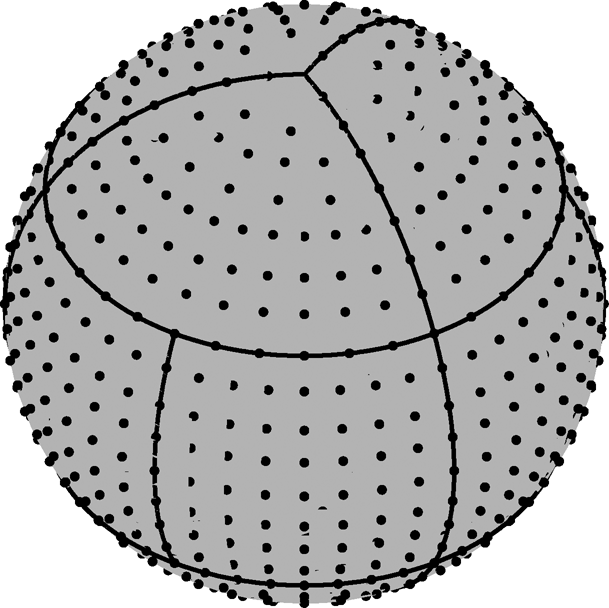
\includegraphics[width=5cm]{afbeeldingen/Directivity_IGLOO.png}
    \caption{Fig. 1 uit \cite{Zhang2012575}. \textit{Picture of the 3:6:3 equal area division, which divides the sphere into 12 base regions, three at either cap and six $60^\circ\times60^\circ$ equatorial regions. Here, each base region is sampled with 64 points.}}
    \label{fig:IGLOO}
\end{figure}

\begin{figure}[h]
    \centering
    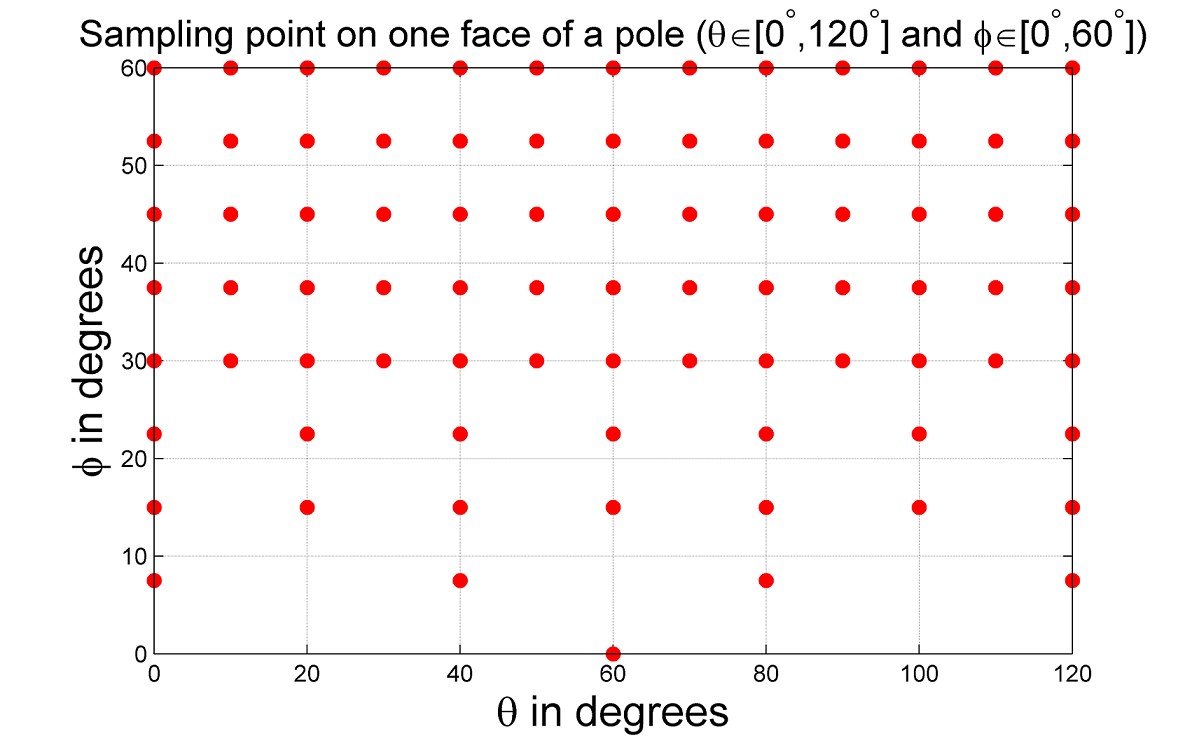
\includegraphics[width=10cm]{afbeeldingen/poolvlak_optimaal.png}
    \caption{Verdeling op poolvlak}
    \label{fig:poolvlak}
\end{figure}

\subsection{Gekozen schema}
Het IGLOO-bemonsteringsschema lijkt dus vooral geschikt voor kleinere hoeken (of grotere bollen), omdat de eisen aan $\Delta\theta$ van gemene deler van 30 en 60 dan makkelijker toepasbaar zijn.
Het bemonsteringsschema dat is gebruikt voor onze metingen is equiangular, omdat deze minder meetpunten nodig heeft dan de IGLOO methode in onze opstelling en nauwkeurig genoeg voor frequenties tot $f_\text{meet}=\dfrac{360\cdot v_\text{lucht}}{2\cdot\Delta\theta\cdot\ell_\text{evenaar}}=\dfrac{360\cdot344}{2\cdot9\cdot0.871}\approx7898$ Hz.

GROTERE BOL TAFELTJE? WAAROM NIET?

INVLOED VOCHTIGHEID EN LUCHTDRUK OP IMPULSE RESPONSE

%-----------------------------------------------------------------------------
\section{Interpolatiemethoden}
Spline interpolation \cite{book:vuik}.